% ================================================================
% Use the following if all authors are from the SAME institution
% ================================================================
\documentclass[accepted,single]{gipaper}

% use Times fonts
\usepackage{times}
% make sure English hyphenation rules, etc. loaded
\usepackage[english]{babel}
% permits inclusion of PNG, JPG, and PDF files under pdflatex
\usepackage{graphics}

% permits figures at bottom of page
\usepackage{dblfloatfix}

\usepackage{epsfig}
\usepackage{newalg}

\usepackage{caption}
\captionsetup[table]{skip=0pt}
\captionsetup[table]{font=small}

% \usepackage{url}
% \bibliographystyle{IEEEtran.bst}

% a more flexible replacement for "verbatim" for typesetting pseudocode
\usepackage{alltt}
% gives automatic table of contents, permits setting PDF
% attributes of document.   Set page size in pdftex.cfg file;
% the "letterpaper" option to hyperref is unreliable...
\usepackage[
    pdftitle = "{Dynamic Bandwidth Allocation with Minimum Rate Guarantees Using OpenFlow}",
    pdfauthor = "{Joel van Egmond}"
]{hyperref}

\title{Dynamic Bandwidth Allocation with Minimum Rate Guarantees Using OpenFlow}

\newauthor{mm}{Joel van Egmond}{}
% Can add more authors
\newauthor{se}{Maryam Elahi}{}
\newauthor{ya}{Mea Wang}{}
%\newauthor{fa}{Fourth Author}{}

% Common affiliation
\affiliation{
    Department of Computer Science \\
    University of Calgary
}

% ================================================================
% Use the following if the authors are from MULTIPLE institutions
% ================================================================
%
% \documentclass[accepted,oneeach]{gipaper}
% \usepackage{graphics}
% \usepackage{hyperref}
%
% \title{Paper Format for CPSC 502/503/601 \\ Instructions to Authors}
%
% \newauthor{wd}{Author One}{Department of Computing Science\\ University of Nowhere}
% \newauthor{se}{Someone Else}{Another Department\\ A Company}
% \newauthor{ya}{Yet Another}{Yet Another Department\\ Another University}
% \newauthor{fa}{Fourth Author}{Department of Computing Science\\ University of Nowhere}
%
% ================================================================
% The rest of the document follows.
% ================================================================

\abstract{ Quality of Service (QoS) control typically refers to network mechanisms used to guarantee a certain service from the network \cite{Krishna:2016}. Many service providers use hard QoS controls to guarantee bandwidth to their clients. In current solutions excess idle bandwidth is wasted, but with the emergence of Software-Defined Networking (SDN) and the OpenFlow protocol, it is possible to program a network to respond to this problem cheaply and efficiently.
This paper describes the design of an SDN/OpenFlow solution that ensures minimum bandwidth guarantees for clients while fairly distributing the excess bandwidth among current users to maximize link capacity utilization.  }

\begin{document}
\begin{keywords}
OpenFlow, Ryu, software defined networking, traffic shaping, quality of service.
\end{keywords}

%------------------------------------------------------------------
% Introduction
%------------------------------------------------------------------
\section{Introduction}
\label{intro}

Quality of Service (QoS) control typically refers to network mechanisms used to guarantee a certain service from the network \cite{Krishna:2016}. Minimum bandwidth is a service frequently guaranteed by QoS. Internet service providers (ISPs) are common users of QoS technology. Traditional ISPs such as Bell, Telus, and Shaw aim to maximize profits and avoid having excess unused bandwidth by overselling their channel to more clients than it can support, with the assumption that not all clients will be using the channel simultaneously. In contrast, many other large-scale service providers, such as the research and education focused Cybera, ORION, and MRnet do not oversell their channel, opting to use QoS controls to guarantee each client that their allocated bandwidth will always be available even if every other client is currently using their own maximum allocated bandwidth. Consequently, these networks often have significant amounts of excess idle bandwidth, since it is very unlikely that every client will be actively using the network at all times. Currently the bandwidth is wasted while the operation and maintenance costs of the full channel must still be paid. This leads to the problem of how to make use of all this excess bandwidth, while still maintaining the minimum bandwidth guarantees demanded by the clients.

Software-Defined Networking (SDN) is an emerging network paradigm that decouples network control and forwarding functions, enabling network control to be directly programmable \cite{opennetworking}. This is done by implementing the network control function in a centralized controller node, which communicates to all the network devices in the network through a standardized protocol. OpenFlow is one such protocol; an open standard protocol that acts as an abstracted switch interface to allow the SDN controller to control the routers/switches in its domain \cite{sdx}.

The purpose of this research is to design and implement an SDN solution to the excess bandwidth problem, in order to maximize the utilization of a network while providing minimum bandwidth guarantees to its clients. This is done by directing network traffic through an OpenFlow enabled switch. The switch is connected to a SDN controller device, which uses the switch's features to guarantee minimum bandwidths while dynamically allocating the excess bandwidth to clients according to a dynamic allocation algorithm, of which three have been developed. The algorithms in question are inspired by common CPU scheduling algorithms, but have been custom designed to approximate the functionality of their inspirations within the limitations of the OpenFlow switch environment.

This research contributes to the body of QoS research by presenting an original SDN/OpenFlow traffic shaping design, which provides both minimum bandwidth as a guaranteed service, as well as the ability to utilize and fairly distribute the excess bandwidth in the link. Once implemented the solution will be evaluated first on its ability to guarantee minimum rates, and then on each algorithm's link capacity utilization and fairness of allocation.

% this figure has to be declared here for some reason or it appears on the wrong page
%\begin{figure*}[!b]
%	\centering
%	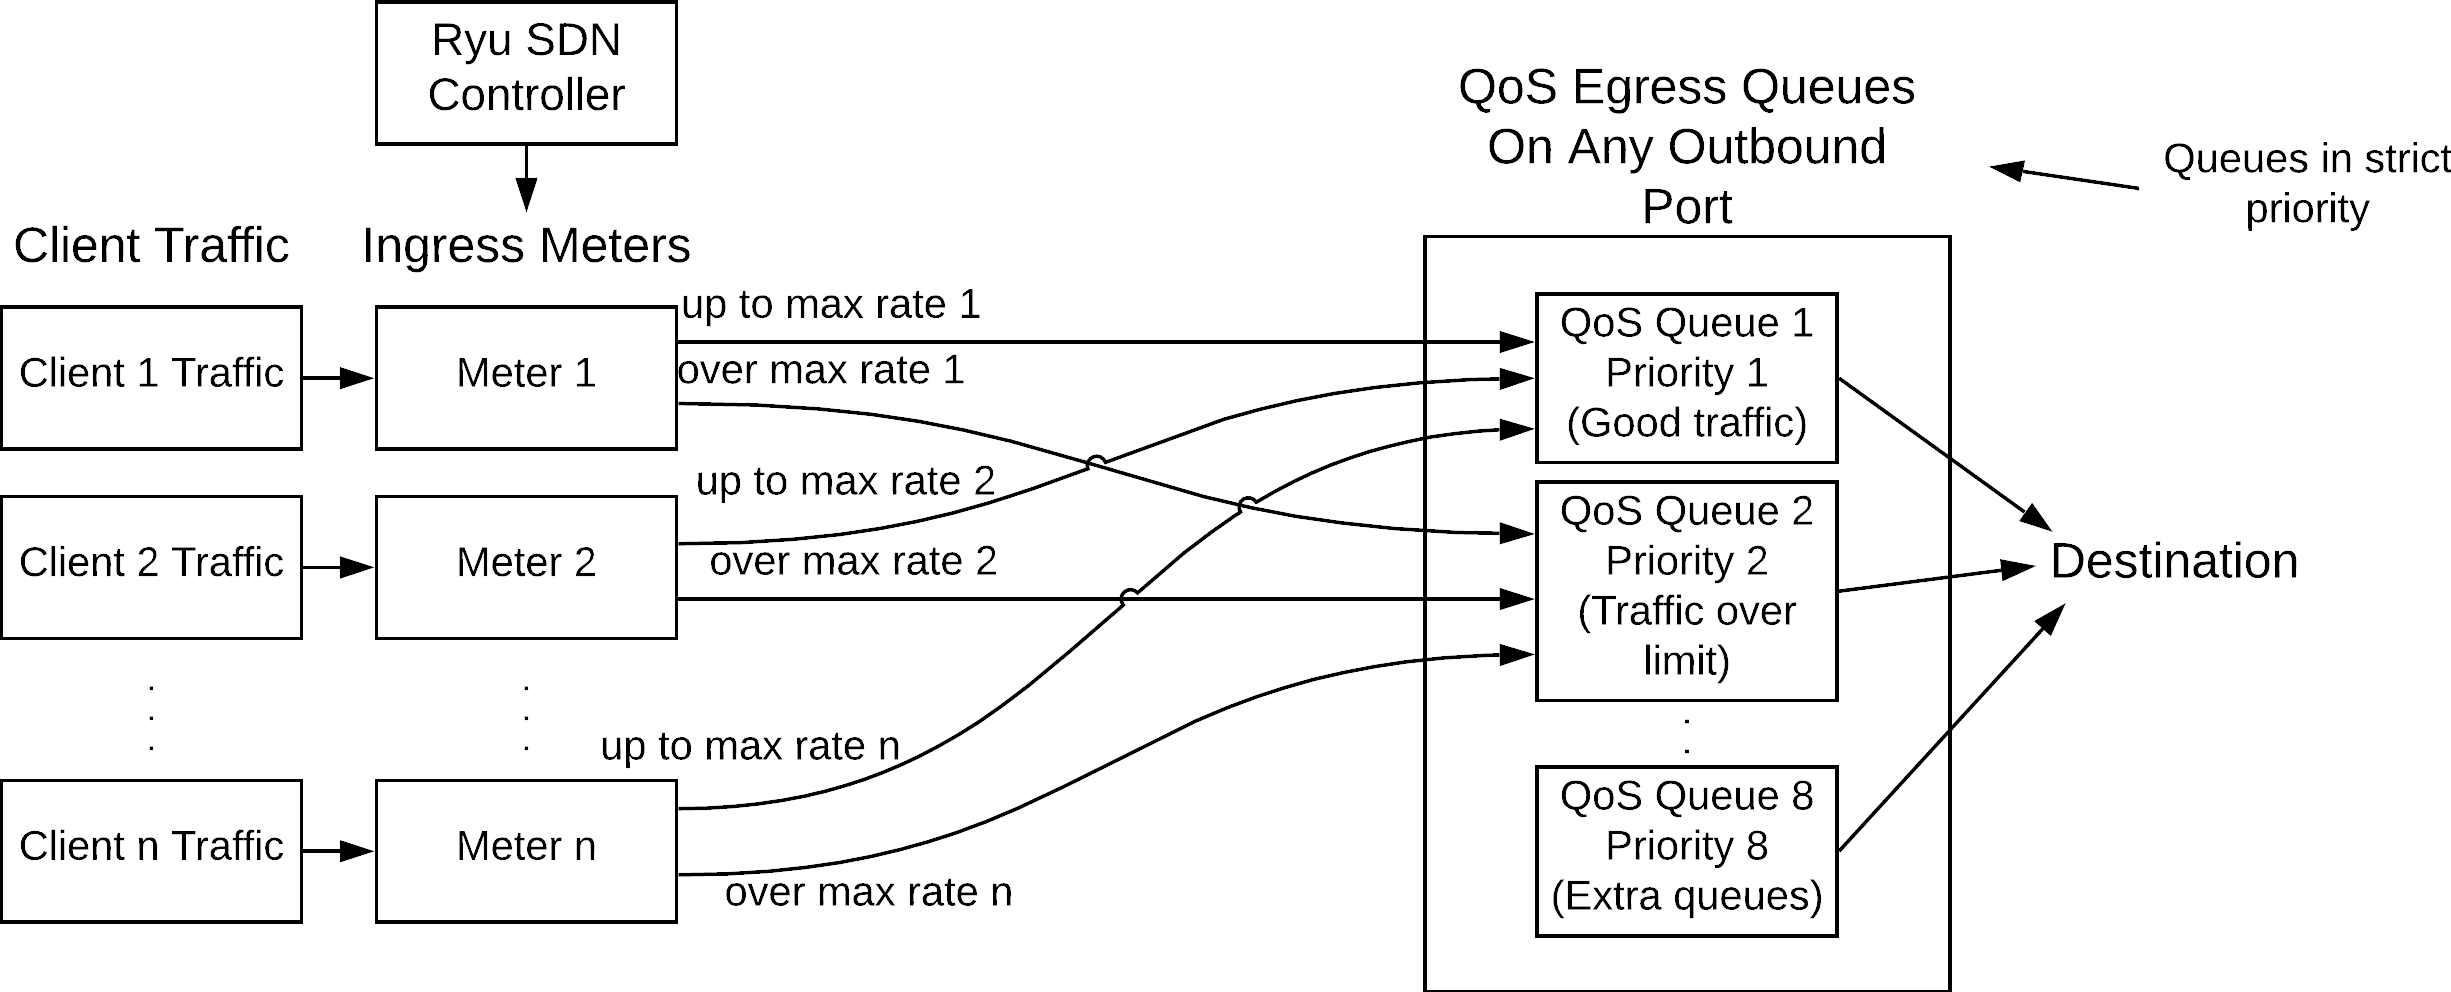
\includegraphics[width=6in]{figs/bwGuar3.png}
%	\caption{ Pica8 setup for minimum bandwidth guarantee. } \label{bwDiag}
%\end{figure*}

\subsection{Key Definitions}
\label{definitions}

When discussing an OpenFlow switch in the context of this research there are several important terms to understand: Flows, meters, meter bands, Differentiated Services Code Point (DSCP) remark, and queues.
\\

In OpenFlow, a flow describes a set of packets transferred from one network endpoint to another endpoint. The endpoints may be defined as IP addresses, TCP/UDP ports, VLAN identifiers, or physical device ports, among others. A flow additionally defines the of rules describing the forwarding actions that the device should take for all packets belonging to that flow \cite{flowdef}. Flows may be manually installed on a switch, or installed by the SDN controller.

Meters are flow monitoring tools which allow the rate monitoring of traffic going into the switch (ingress traffic). Meters are attached to specific flows, and can perform operations based on the rate of traffic entering those flow, specifically dropping or DSCP remarking packets.

Meter bands are a feature of meters that allow them to perform operations on traffic in a flow. A meter band defines a rate threshold and an action, such that when the rate of traffic passing through the meter passes that threshold, the action is applied to all traffic over the threshold.

DSCP remark is a possible action that can be chosen for a meter band. The DSCP remark action is provided a 6-bit value, and will write that value to the Type of Service (TOS)/DSCP field in the IP header of all packets that trigger the meter band. This is important because flows are able to match on the DSCP field, allowing for traffic differentiation.

Finally, queues are the complements to meters for traffic leaving the switch (egress traffic). They are also attached to specific flows, and all traffic passing through the flow is placed into the attached queue. The packets in the queue are then processed at specified minimum and/or maximum rates. On most switches queues are given a priority and are serviced strictly according to their priority, but some switches have support for other queueing algorithms such as round-robin or weighted round-robin.


%commented out
\iffalse
%------------------------------------------------------------------
% Previous Work
%------------------------------------------------------------------
\section{Old Previous Work}
\label{oprev_work}

Previous work that has been conducted relating to this project is focused various methods of using OpenFlow enabled switches to obtain minimum bandwidth guarantees. These focused on two main paradigms: hard guarantees and soft guarantees \cite{softqos}. A hard bandwidth guarantee uses a static reservation of network resources for the specified traffic, whereas a soft bandwidth guarantee uses a differentiated service approach with no reservation, in which some traffic is given priority over other traffic using only currently available network resources. 

\subsection{Hard Guarantee}
\label{prev_hard_qos}

In a 2014 paper, Tomovic et al. \cite{Tomovic:2014} proposed a system with hard QoS guarantees using OpenFlow. The hard guarantee is established by forcing all flows to request bandwidth on the link. The SDN controller evaluates each request and allocates bandwidth to the requesting flow if there is capacity on the link, otherwise the request is rejected. Once allocated, the bandwidth is reserved for exclusive use by that flow until the flow expires. The guarantee is implemented on the switch level by installing an egress queue with minimum and maximum bandwidth equal to the guaranteed bandwidth.

In a later paper, Dwarakanathan et al. \cite{Dwara:2015} designed a similar hard QoS system also using OpenFlow, with the goal of using less queues. Instead of creating one queue per guaranteed flow as in Tomovic's \cite{Tomovic:2014} system, it instead uses only one queue shared between all guaranteed flows, whose minimum and maximum are dynamically adjusted as bandwidth requests are granted and previously granted flows expire.

In both of these systems, the maximum rate is equal to the guaranteed rate, preventing the flow from ever exceeding its guaranteed rate. This means that any unreserved bandwidth goes unused, resulting in sub-optimal link capacity utilization. They also both rely on all nodes in the network between the start and end points allocating resources, which introduces scalability difficulties. 

\subsection{Soft Guarantee}
\label{prev_soft_qos}

In their 2013 paper, Wallner and Cannistra \cite{Wallner:2013} implemented a soft QoS system using the Floodlight SDN controller. The paper presents a proof of concept model for class-based QoS control. First, incoming packets are classified based on their ToS/DSCP bits in the IP header. Then, class-based priority traffic shaping is implemented in switches along the path using egress queues.

In a paper closely linked to this project, Krishna et al. \cite{Krishna:2016} designed a hybrid soft QoS which used an OpenFlow enabled switch to allow QoS flows to guarantee a minimum rate while still being able to send more than their guaranteed rates, as long as they do not hinder other guaranteed and/or best-effort flows. The system classifies packets similar to Wallner and Cannistra's \cite{Wallner:2013}, but will only prioritize traffic up to their guaranteed minimum rate. Excess traffic is given lower priority and transmitted on a first-come first-serve basis. Additionally, this system in only needs to be implemented in a single switch, easing the scalability difficulties.

In Wallner and Cannistra's \cite{Wallner:2013} system minimum rates are only guaranteed by class and not by individual client, and in both systems the excess bandwidth is only distributed on a first-come first-serve basis, allowing clients with high traffic to unfairly dominate the channel.
\\\\
All these models implement bandwidth guarantees, but with shortcomings in the areas of link capacity utilization (in hard guarantees) and fairness of bandwidth distribution (in soft guarantees). This project will address these shortcomings by allowing excess link capacity to be used, and dynamically allocating the excess bandwidth fairly.
\fi


%------------------------------------------------------------------
% Previous Work
%------------------------------------------------------------------
\section{Previous Work}
\label{prev_work}

The body of existing research relevant to this project can be classified in four major sections: hard guarantees, soft guarantees, flow monitoring, and scheduling algorithms. The first two sections refer to the two main paradigms that have emerged from the various methods of using OpenFlow enabled switches to obtain minimum bandwidth guarantees. A hard bandwidth guarantee uses a static reservation of network resources for the specified traffic, whereas a soft bandwidth guarantee uses a differentiated service approach with no reservation, in which some traffic is given priority over other traffic using only currently available network resources \cite{softqos}. The third sections refers to methods of monitoring network traffic passing through OpenFlow flows. The final section refers to various network packet scheduling algorithms and discussions on their efficiency and fairness.

\subsection{Hard Guarantee}
\label{hard_qos}

Designing methods of achieving hard bandwidth guarantees was the focus of research by Tomovic et al. \cite{Tomovic:2014} and Dwarakanathan et al. \cite{Dwara:2015}.
\\


Tomovic et al. \cite{Tomovic:2014} argue that providing QoS guarantees to applications is an important objective of modern networks. With the rising popularity of real-time applications, especially in multimedia, the need arises for a network service model with performance guarantees. Current models (such as IntServ and DiffServ) lack adequate control, so QoS is currently often implemented by assigning separate physical networks with their own hardware to each class of traffic, incurring high operational expenditures and infrastructure costs. The paper aims to address this issue by designing a Software-Defined Networking (SDN) control environment to provide bandwidth guarantees between two points. The solution works by shifting network intelligence into a PoX SDN controller, which accepts/denies bandwidth requests, monitors network resources, and calculates traffic routes \cite{Tomovic:2014}. The solution is evaluated through a pair of experiments, which aim to demonstrate that the system can actually provide the minimum bandwidth guarantees between two points in the work. IntServ has been chosen as a baseline, and the results of each experiment are compared this baseline to measure improvement. This paper contributes to the body of QoS research by demonstrating the design of an SDN/OpenFlow control environment that provides bandwidth guarantees for priority flows in an automated manner, alleviating the need for distinct physical networks for multiple classes of service.


Dwarakanathan et al. \cite{Dwara:2015} argue that current QoS solutions are not sufficiently scalable. To address this they implemented a similar SDN environment to that of Tomovic et al. \cite{Tomovic:2014}, using a Floodlight SDN controller as the point of network intelligence instead of a PoX controller. Dwarakanathan's \cite{Dwara:2015} solution aims to be more scalable than that of Tomovic et al. \cite{Tomovic:2014} by using fewer queues in each switch. Instead of creating one queue per guaranteed flow as in Tomovic's \cite{Tomovic:2014} system, it instead uses only one queue shared between all guaranteed flows, whose minimum and maximum are dynamically adjusted as bandwidth requests are granted and previously granted flows expire. The solution is evaluated through experiments ran in the Mininet simulator, in which theoretical minimum rates are calculated and compared against the experimental results. This paper contributes to the body of QoS research by demonstrating that it is possible to create a scalable QoS solution with SDN.


In all of these systems, the maximum rate is equal to the guaranteed rate, preventing the flow from ever exceeding its guaranteed rate. This means that any unreserved bandwidth goes unused, resulting in sub-optimal link capacity utilization. They also both rely on all nodes in the network between the start and end points allocating resources, which introduces scalability difficulties.

\subsection{Soft Guarantee}
\label{soft_qos}

Designing methods of achieving soft bandwidth guarantees was the focus of research by Krishna et al. \cite{Krishna:2016} and Wallner and Cannistra \cite{Wallner:2013}.
\\


Krishna et al. \cite{Krishna:2016} argue that QoS is currently underutilized in provider networks, because it is too complicated to install and maintain. A response to this issue would be of great interest to large-scale internet service providers, who currently massively overprovision their networks at great cost. This paper aims to demonstrate how to use Software-Defined Networking (SDN) and the OpenFlow protocol’s QoS features to cheaply and efficiently implement minimum bandwidth guarantees in a network. The solution described in the paper uses a Ryu SDN controller communicating with an OpenFlow enabled switch, through which all QoS traffic will pass \cite{Krishna:2016}. The minimum bandwidth guarantee is applied by using a combination of the switch’s ingress meter table, and and egress queues. The ingress meters are used to aggregate traffic and redirect packets over the guaranteed minimum rate, and the egress queues and used to ensure priority traffic is transmitted first. The success of their solution is measured by the results of their three experiments. The first experiment tests the creation of new QoS flows in the system, the second tests traffic aggregation and prioritization, and the the third tests the responsiveness of the system. The experiments all have calculated theoretical expected results, and the effectiveness of the system is measured by how close the actual results come the expected results. The key metrics analyzed are bandwidth use for each flow, bandwidth use of the full channel, and time to adjust to changes in bandwidth usage. The paper contributes to the body of QoS knowledge by demonstrating how to implement minimum bandwidth guarantees using OpenFlow, while still allowing excess bandwidth to be shared without causing packet loss.


Wallner and Cannistra \cite{Wallner:2013} argue that different network services (such as Voice Over IP (VOIP), stored video streaming, and live video streaming) have different requirements in terms of latency and bandwidth, and that these services can be divided into classes based on these requirements. Their paper addresses this by presenting a proof of concept model for class-based QoS control using SDN. A floodlight SDN controller is used to control many switches in a network, and in each switch incoming packets are classified based on their Type of Service (ToS) bits in the IP header. From this point different classes are given different priorities as they leave the switch. In this system minimum rates are only guaranteed by class and not by individual client, and the excess bandwidth is only distributed on a first-come first-serve basis. The effectiveness of this solution is unclear, as no empirical methods of evaluation are mentioned in the paper. The paper contributes to the body of QoS research by demonstrating that it is possible to use SDN to implement class-based QoS.


In Wallner and Cannistra's \cite{Wallner:2013} system minimum rates are only guaranteed by class and not by individual client, and in both systems the excess bandwidth is only distributed on a first-come first-serve basis, allowing clients with high traffic to unfairly dominate the channel.


\subsection{Flow Monitoring}
\label{flow_monitor}

Designing methods of performing real-time monitoring of flow statistics was the focus of a paper by van Adrichem et al. \cite{vanAdrichem}.
\\


Van Adrichem et al. \cite{vanAdrichem} argue that a key requirement to implement effective QoS in an SDN network is accurate traffic monitoring, on a finely-grained (per flow) basis. They state that current flow-based measurement techniques are too resource hungry in terms of CPU and bandwidth usage. To address this issue they propose \textit{OpenNetMon}, a POX OpenFlow controller module enabling accurate monitoring of per-flow throughput, packet loss and delay metrics \cite{vanAdrichem}. \textit{OpenNetMon} improves upon current measurement techniques by optimizing the choice of which switches are polled, and the frequency which they are polled, in order to minimize network resource usage while maintaining high accuracy \cite{vanAdrichem}. \textit{OpenNetMon}'s effectiveness was evaluated by running an \textit{OpenNetMon} module as well as \textit{tcpstat} on a node, and comparing their monitoring statistics as well as CPU and bandwidth usage. This paper contributes to the body of SDN research by demonstrating that is is possible to efficiently perform per-flow monitoring.


\subsection{Scheduling Algorithms}
\label{algs}

Design, and evaluation of network scheduling algorithms was the focus of a paper by Balogh et al. \cite{Balogh}.
\\


Balogh et al. \cite{Balogh} argue that in a networking ecosystem that is increasingly making use of class-based priority QoS, the way how waiting packets in network nodes are selected for output is a significant factor for providing that QoS. In their paper they investigate three priority queuing based scheduling algorithms. The algorithms are Priority Queuing (PQ), Weighted Round Robin with Priority Queueing (WRRPQ), and Low Latency Queuing (LLQ) \cite{Balogh}. These algorithms all support strict priority queueing, in which time critical priority data can be transmit first. PQ is a simple strict priority algorithm, in which priority packets are sent first, and all other packets are sent in first-come first-serve \cite{Balogh}. WRRPQ is a combination of PQ and Weighted Round Robin, in which priority packets are sent first, and other packets are sent according to Weighted Round Robin \cite{Balogh}. LLQ is an algorithm which considers the time required to send each packet to minimize latency \cite{Balogh}. The algorithms were evaluated by testing each one in a simulated network using different kinds of traffic. The results found that effectiveness of each algorithm depended on the kind of traffic (LLQ better for VOIP, WRRPQ better for fixed size packets). This paper contributes to the body of QoS research by showing that there are different optimal priority queuing algorithms for class-based QoS depending on the type of traffic.
\\\\


\label{prev_work_conclusion}
All these models implement bandwidth guarantees, but with shortcomings in the areas of link capacity utilization (in hard guarantees) and fairness of bandwidth distribution (in soft guarantees). This project addresses these shortcomings by allowing excess link capacity to be used, and dynamically fairly allocating the excess bandwidth.


%commented out
\iffalse
%------------------------------------------------------------------
% Solution
%------------------------------------------------------------------
\section{Solution}
\label{solution}

This project aims to implement a hybrid soft/hard QoS system, in which minimum bandwidth is given a hard guarantee for each client, and excess bandwidth is available for use. It will address the shortcomings of previous work by including dynamic allocation of the excess bandwidth beyond only first-come first-serve, and functioning as a single-switch solution.

\subsection{Minimum Bandwidth Guarantee}
\label{sol_min_band}

The minimum bandwidth guarantee will be achieved through a similar method to Krishna’s \cite{Krishna:2016} system. It will be implemented using an OpenFlow enabled switch, using egress queues, ingress meters, and an SDN controller remotely controlling the switch. The egress queues will be set in a strict priority system, in which the higher priority queue always goes first. The highest priority queue will be used for guaranteed rate traffic, and the lower priority queues will be used for traffic over clients’ guaranteed minimum rates. The ingress meters will be used for traffic aggregation and setting the minimum rate for each client. Each individual client will have a meter assigned to them, which will measure incoming/outgoing traffic. The meter will direct all traffic under the guaranteed bandwidth (meter maximum rate) to the highest priority queue, ensuring that it will be transmitted first. All traffic over the guaranteed rate will be redirected to the lower priority queues, depending on the dynamic allocation algorithm being used. This redirection will guarantee the minimum rate for each client so long as the system obeys the equation:

\begin{eqnarray*}
	\sum M_{max} &\leq& R
\end{eqnarray*}

Where $M_{max}$ is a meter maximum rate, and $R$ is the link transmission rate. This is to say the minimum rates will always be guaranteed so long as the sum of the minimum rates is not greater than the maximum link rate.

\subsection{Dynamic Bandwidth Allocation}
\label{sol_dynamic_alloc}

Once bandwidth guarantees are implemented, the rest of the excess bandwidth will need to be distributed. This will be done by implementing various distribution algorithms in the SDN controller. The controller will read real-time bandwidth usage for each client from the meters and adjust how the traffic is redirected dynamically according to what algorithm is in use. 

The design required for bandwidth guarantees puts some restrictions on algorithm design. Only the ingress meter settings can be changed dynamically, and the egress queues have a strict priority system, meaning the higher priority will always transmit first. This means that it is non-trivial to implement any dynamic allocation algorithm outside first-come first-serve, even an algorithm as simple as round robin will require some creativity to implement while maintaining the bandwidth guarantees. Accordingly, the three planned allocation solutions are relatively simple: egalitarian fairness, proportional fairness, and hybrid proportional fairness.

In egalitarian fairness, an equal share of the excess bandwidth is given to all members upon demand. This aims to treat all members as equals regardless of the minimum service they use. This solution is inspired by the round robin scheduling algorithm.

%commented out
\iffalse
In egalitarian fairness (Table 1), an equal share of the excess bandwidth is given to all members upon demand. This solution is inspired by the round robin scheduling algorithm. \\

\begin{table}[htpb]
	\label{egalitarian_table}
	\vspace{-3mm}
	\begin{center}
		\begin{small}
			\begin{tabular}{cccc}
				%\hline
				Client & Minimum & Demand & Allocation \\
				\hline
				Client 1 & 100 & 300 & 200 \\
				Client 2 & 200 & 400 & 300 \\
				Client 3 & 300 & 500 & 400 \\
			\end{tabular}
		\end{small}
	\end{center}
	\caption{Example of egalitarian fairness (Total bandwidth: 900 Mbps)}
	\vspace{-3mm}
\end{table}
\fi

In proportional fairness, the share of the excess bandwidth given to each member upon demand is in proportion to its allocated minimum bandwidth guarantee. This aims to give members attributed a higher minimum service a better share of the excess bandwidth.This solution is inspired by weighted round robin scheduling algorithm.

%commented out
\iffalse
In proportional fairness (Table 2), the share of the excess bandwidth given to each member upon demand is in proportion to its allocated minimum bandwidth guarantee. This solution is inspired by weighted round robin scheduling algorithm. \\

\begin{table}[htpb]
	\label{proportional_table}
	\vspace{-3mm}
	\begin{center}
		\begin{small}
			\begin{tabular}{cccc}
				%\hline
				Client & Minimum & Demand & Allocation \\
				\hline
				Client 1 & 100 & 300 & 150 \\
				Client 2 & 200 & 400 & 300 \\
				Client 3 & 300 & 500 & 450 \\
			\end{tabular}
		\end{small}
	\end{center}
	\caption{Example of proportional fairness (Total bandwidth: 900 Mbps)}
	\vspace{-3mm}
\end{table}
\fi

In hybrid proportional fairness, each member has priority to use the excess bandwidth up to a fraction of its allocated minimum bandwidth, and the remainder is equally shared. This aims to give preference to higher usage members as in proportional fairness, but with a limitation that prevents them from dominating the channel.

%commented out
\iffalse
In hybrid proportional fairness (Table 3), each member has priority to use the excess bandwidth up to a fraction of its allocated minimum bandwidth, and the remainder is equally shared. \\

\begin{table}[h]
	\label{hybrid_table}
	\vspace{-3mm}
	\begin{center}
		\begin{small}
			\begin{tabular}{cccc}
				%\hline
				Client & Minimum & Demand & Allocation \\
				\hline
				Client 1 & 100 & 300 & 190 \\
				Client 2 & 200 & 400 & 300 \\
				Client 3 & 300 & 500 & 410 \\
			\end{tabular}
		\end{small}
	\end{center}
	\caption{Example of hybrid proportional fairness (Total bandwidth: 900 Mbps, 1/10th of minimum prioritized )}
	\vspace{-3mm}
\end{table}
\fi

The details of how each of these solutions will be implemented is yet to be determined, but they will be evaluated on their link capacity utilization and fairness. Without any dynamic solution, the system will behave as though first-come first-serve was implemented, so this will be the baseline to compare against.
\fi

%------------------------------------------------------------------
% Methodology
%------------------------------------------------------------------
\section{Methodology}
\label{methodology}

This project implements a hybrid soft/hard QoS system, in a two-part solution. The first part of the solution is to achieve a minimum bandwidth guarantee for each client while retaining the use of the excess bandwidth on a first-come first-serve basis. The second part of the solution addresses the dynamic fair allocation of the excess bandwidth beyond only first-come first-serve. Both parts of the solution are implemented using an OpenFlow enabled Pica8 switch, with a Ryu SDN controller managing the details of the switch's flows, meters, and queues.

\subsection{Technical Limitations}
\label{tech_limitations}

The unfortunate reality of implementing on a real switch is that OpenFlow is only a standard, and switch manufacturers may not correctly or completely implement the standard. This becomes increasingly apparent when taking advantage of OpenFlow's more recent or esoteric features. While most OpenFlow features work as expected on the Pica8, there are a few limitations that impacted the solution design or required workarounds. The specific problematic limitations are as follows: 

\begin{itemize}
\item The OpenFlow standard supports an arbitrary number of queues, whereas the Pica8 switch only supports 8 queues. This is a realistic hardware limitation, but it imposes scalability restrictions.
\item The OpenFlow standard supports an arbitrary number of meter bands, whereas the Pica8 switch only supports two meter bands. This is also a realistic hardware limitation, but it significantly limits the potential utility of meters.
\item The OpenFlow standard states that the DSCP remark meter action should occur before the flow action of its attached flow. On the Pica8 the DSCP remark action and the flow action happen in parallel. In most cases this results in the same behaviour, except when the flow action is to direct the packet to another set of flows. According to OpenFlow the packet should be remarked and then sent to the next set of flows, allowing the next set of flows to match on the remarked field. In reality the remark is not applied until the packet leaves the switch, and the next set of flows will not be able to match on the remarked field. This is a significant departure from the intended functionality and requires a substantial workaround.
\end{itemize}

The details of the design changes resulting from these limitations are mentioned in the solution descriptions. 

\subsection{Minimum Bandwidth Guarantee}
\label{min_bandwidth}


The minimum bandwidth guarantee was initially planned to be achieved through a system in which each client would have a corresponding meter and queue assigned to them, with one best effort queue to handle excess traffic (Figure 1). The meter would use one meter band set to the client's minimum allocated bandwidth. All traffic under the client's minimum rate would be put into its corresponding flow, while all excess traffic would be DSCP remarked by the meter and directed to the best effort queue. Each client's queue's minimum rate would be set to the client's allocated rate, guaranteeing that the client would never go below that rate. Any excess bandwidth would be used for traffic in the excess traffic queue, allowing for the use of the excess bandwidth. While promising, this system was abandoned because it was not scalable, as for $n$ clients it would require $n+1$ queues, and the Pica8 switch can only support 8 queues.\\

\begin{figure*}
	\centering
	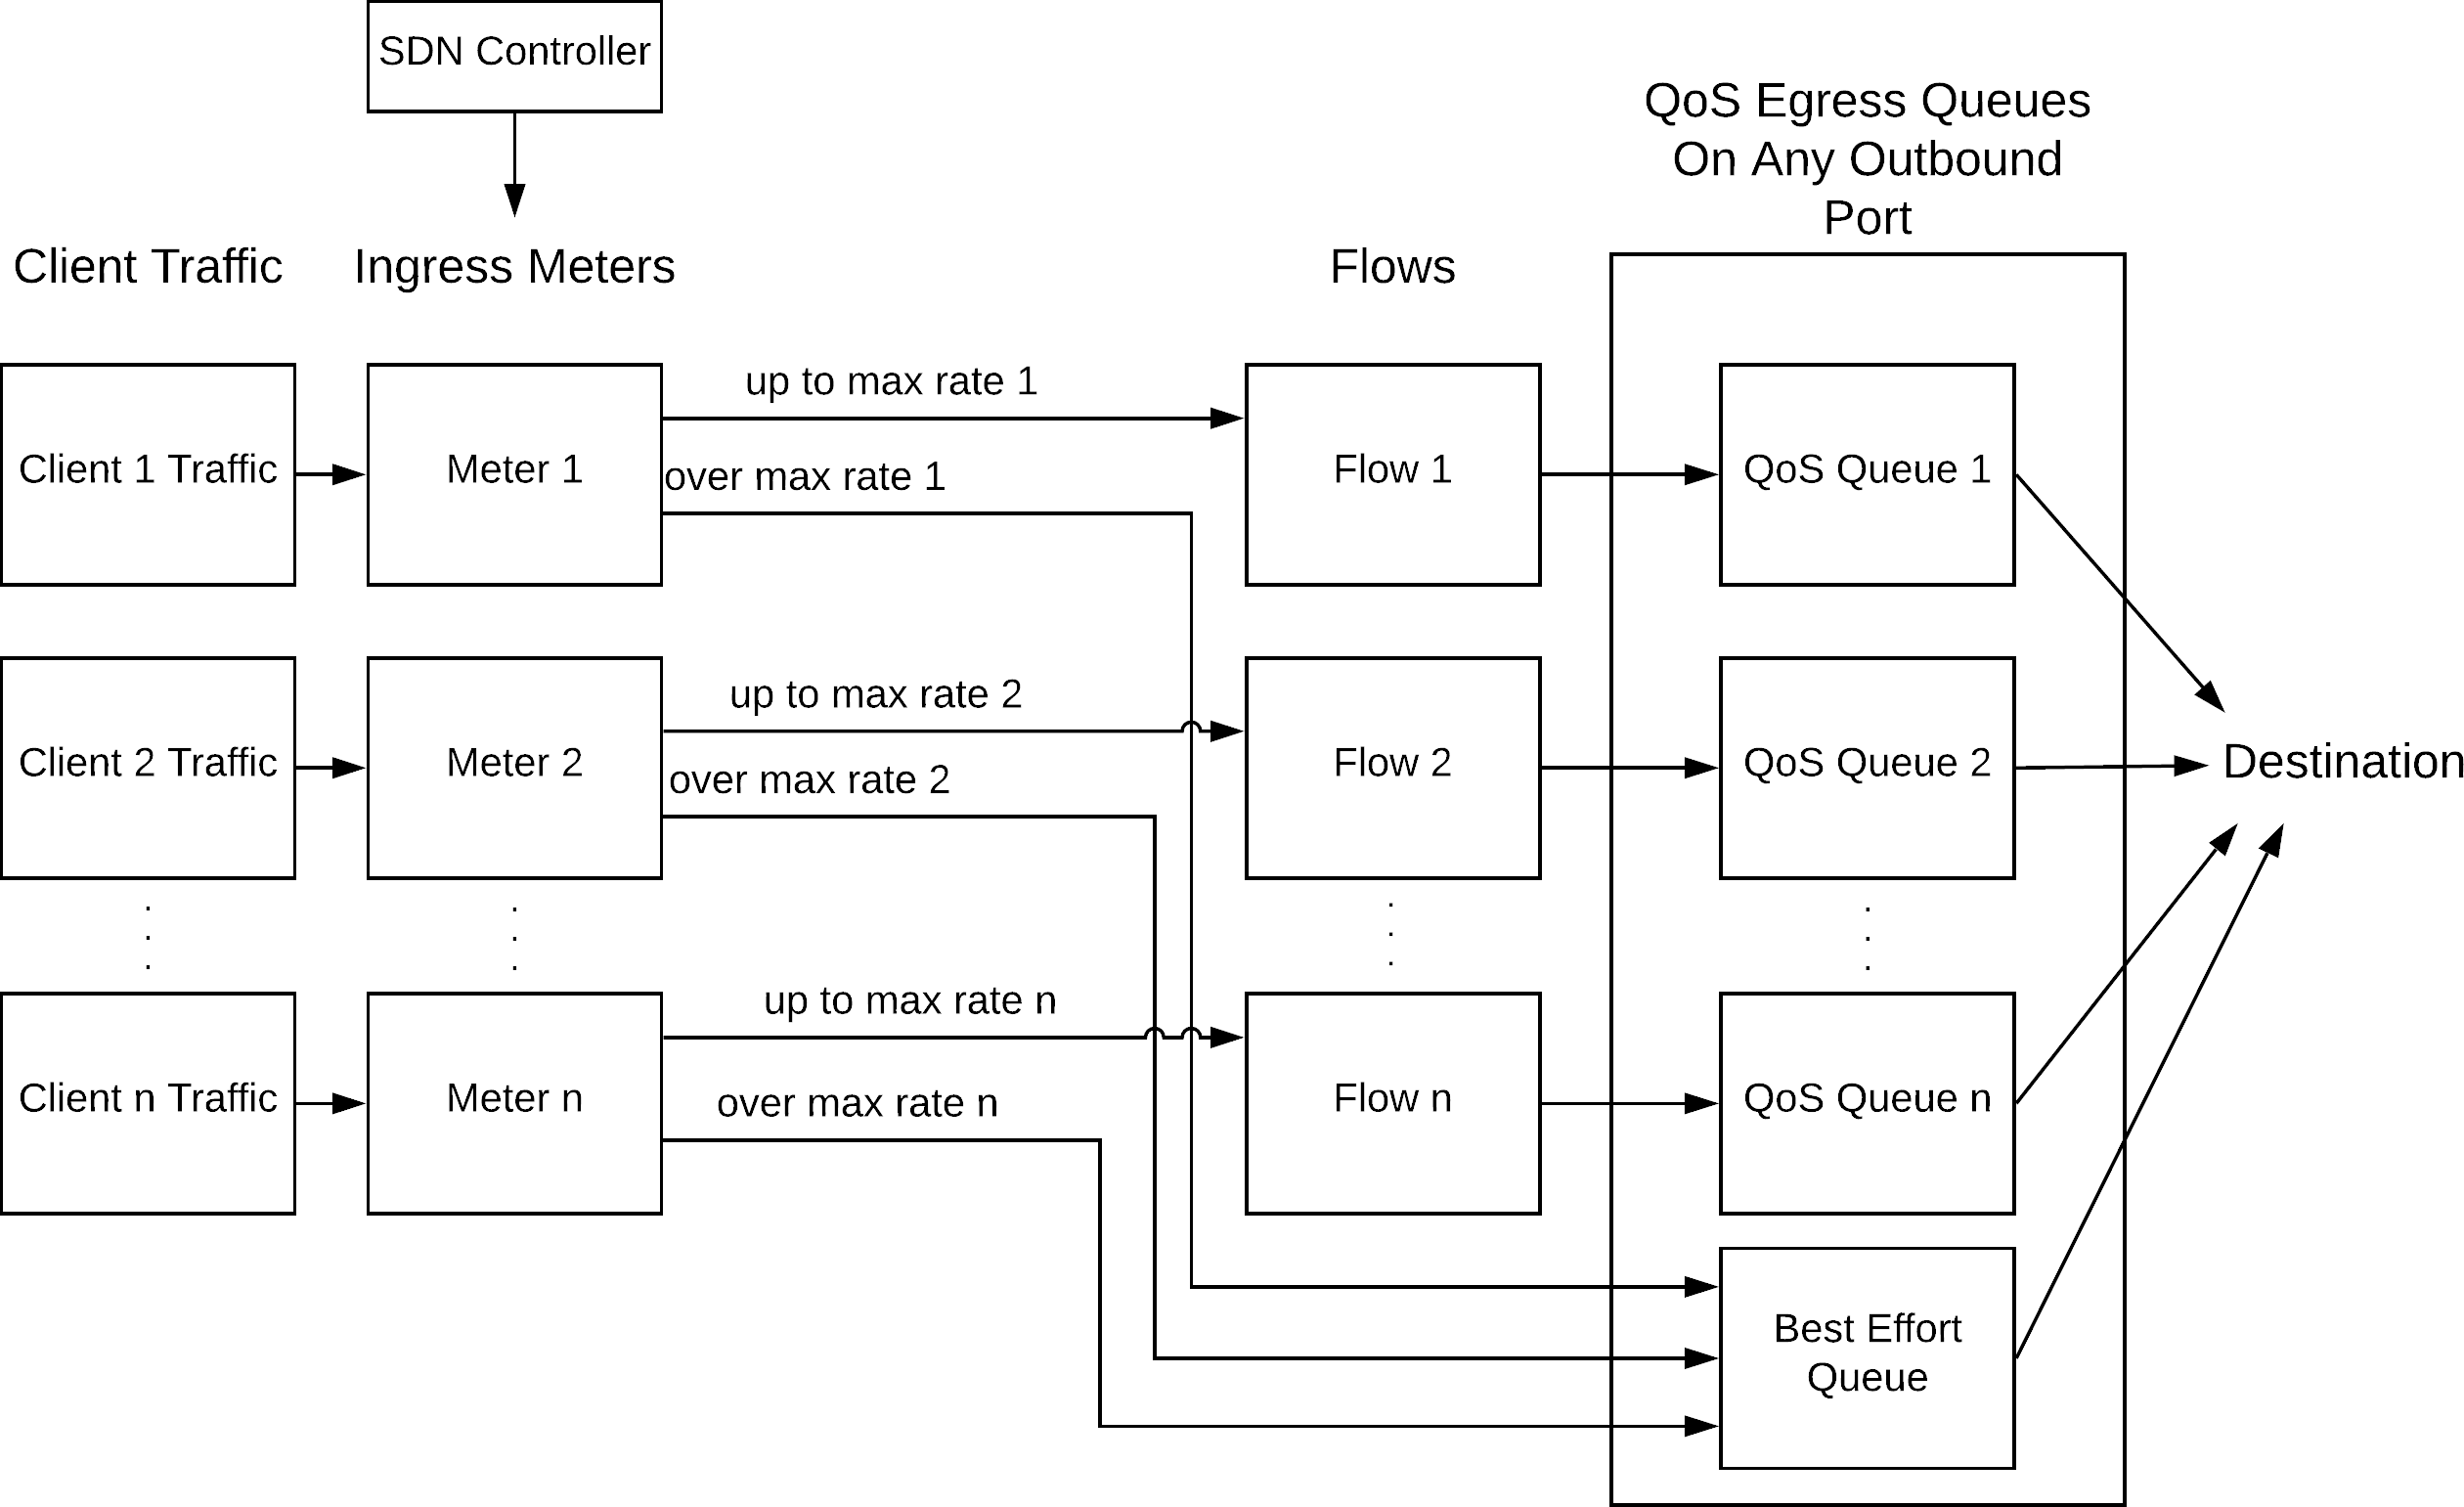
\includegraphics[width=6in]{figs/bwGuar_v1.png}
	\caption{ Initial Pica8 setup for minimum bandwidth guarantee. } \label{bwDiag1}
\end{figure*}

To address the scalability issue, the minimum bandwidth guarantee design was reworked to use a similar method to Krishna’s \cite{Krishna:2016} system (Figure 2). It was implemented using an OpenFlow enabled Pica8 switch, using egress queues, ingress meters, and a Ryu SDN controller remotely controlling the switch. The egress queues are set in a strict priority system, in which the higher priority queue always goes first. The highest priority queue is used for guaranteed rate traffic, and the lower priority queues are used for traffic over clients’ guaranteed minimum rates. The ingress meters are used for traffic aggregation and setting the minimum rate for each client. Each individual client has a meter assigned to them, which measures incoming/outgoing traffic. The meter directs all traffic under the guaranteed bandwidth (meter maximum rate) to the highest priority queue, ensuring that it will be transmitted first. All traffic over the guaranteed rate is DSCP remarked and directed to a second set of flows, which redirected to the lower priority queues by matching on the packets' remarked DSCP field. This redirection guarantees the minimum rate for each client so long as the system obeys the equation:

\begin{eqnarray*}
	\sum M_{max} &\leq& R
\end{eqnarray*}

where $M_{max}$ is a meter maximum rate, and $R$ is the link transmission rate. This is to say the minimum rates will always be guaranteed so long as the sum of the minimum rates is not greater than the maximum link rate. This solution requires a minimum of only two queues for n clients, addressing the initial design's scalability issue.


\begin{figure*}
	\centering
	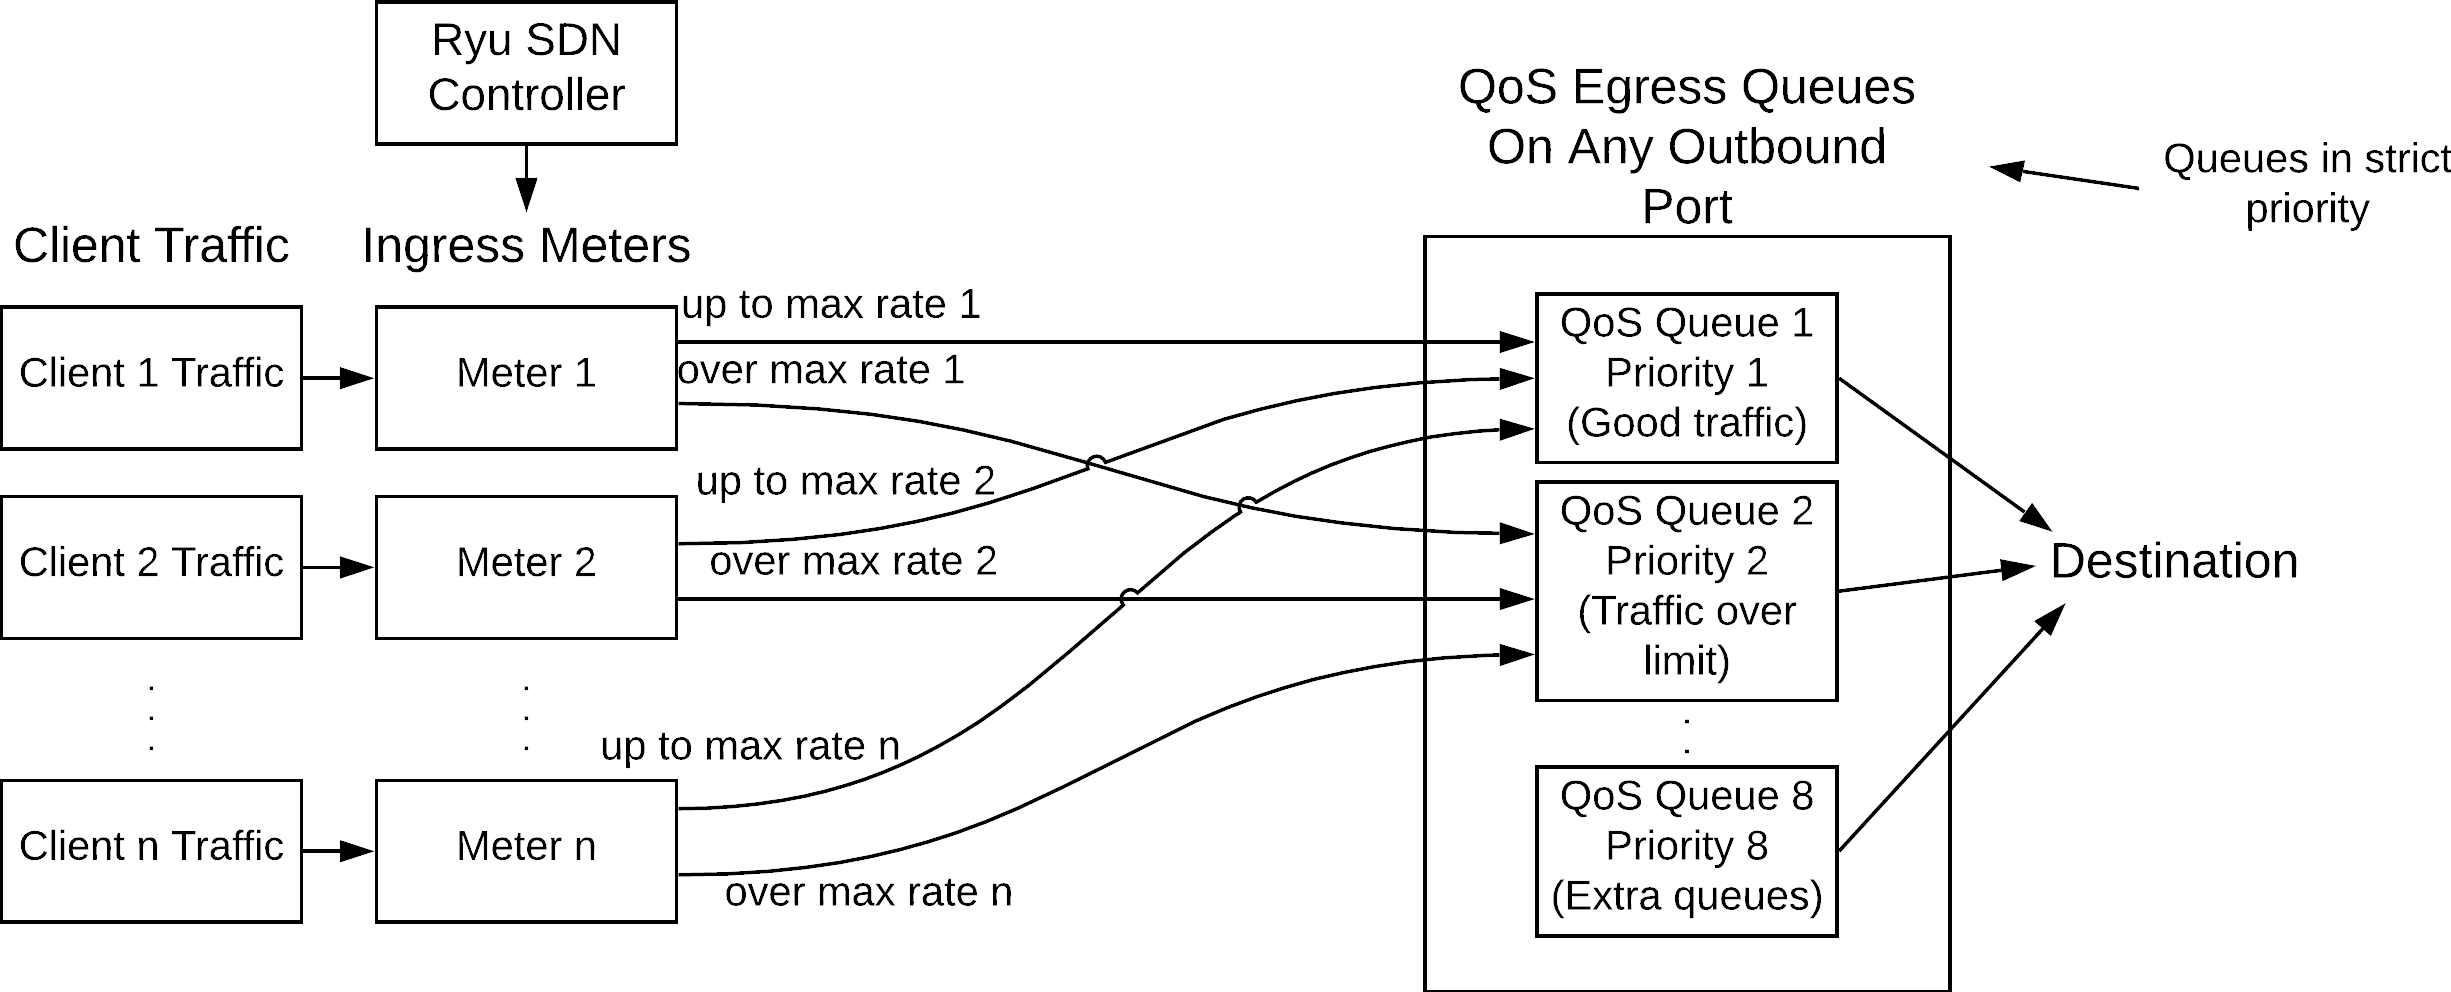
\includegraphics[width=6in]{figs/bwGuar_v2.png}
	\caption{ Modified Pica8 setup for minimum bandwidth guarantee. } \label{bwDiag2}
\end{figure*}

Unfortunately the second design was also subject to a technical limitation, as using DSCP remark to redirect traffic to lower priority queues did not perform as expected, due to the Pica8's aforementioned incorrect implementation of DSCP remark. Since the DSCP remark would still apply after the packet left the switch, the issue was resolved by routing remarked traffic to a second Pica8 switch, and installing the egress queues and second set of flows on the second switch instead of the first. This workaround treats the two switches combined as one entity, with the first switch functioning as the ingress point performing the metering and DSCP remark, and the second switch functioning as the egress point redirecting remarked packets to their appropriate queues.


\subsection{Dynamic Bandwidth Allocation}
\label{min_bandwidth}


Having implemented minimum bandwidth guarantees, the second part of the solution is the ability to distribute the excess bandwidth. This is done by implementing various distribution algorithms in the SDN controller. The controller reads real-time bandwidth usage for each client from the flows and adjusts how the traffic is redirected dynamically according to what algorithm is in use. This system builds onto the guaranteed bandwidth solution by adding another meter band for each meter, and one more queue to the switch (Figure 3). The first meter band's trigger rate is set to the the client's guaranteed minimum bandwidth, sending all traffic under this rate to the high priority queue. The second meter band's trigger rate is set higher than the minimum bandwidth, but is not fixed. Traffic above the first band's rate but below the second band's rate is sent to the medium priority queue. Traffic above the second band's rate is sent to the low priority queue. This creates a three tier priority differentiation of traffic, the first tier for guaranteed traffic, the second tier for dynamically allocated excess traffic, and the third tier for extreme excess traffic. What the second meter band's trigger rate is set to depends on the dynamic allocation algorithm in use, but all algorithms will have some common elements. In each algorithm the SDN controller repeatedly polls the switch flows for their bandwidth usage, allowing the controller to determine the current demanded rate for each client. With this information the controller calculates the amount of excess bandwidth available, and divides it among the currently active clients depending on their current demand and the chosen dynamic bandwidth algorithm. The division is done by setting the second meter bands' trigger rates such that for all clients the sum of the bandwidth captured in the second tier of traffic is equal to the current excess bandwidth available in the link. The controller frequently repeats this process to continuously adapt the system to changing traffic demands, and in this fashion dynamically allocates the excess bandwidth. Because this is a reactive system, the third tier of traffic (extreme excess) exists to capture traffic that the controller has not yet compensated for, ensuring that no packets are dropped and the demand polling remains accurate. 

\begin{figure*}
	\centering
	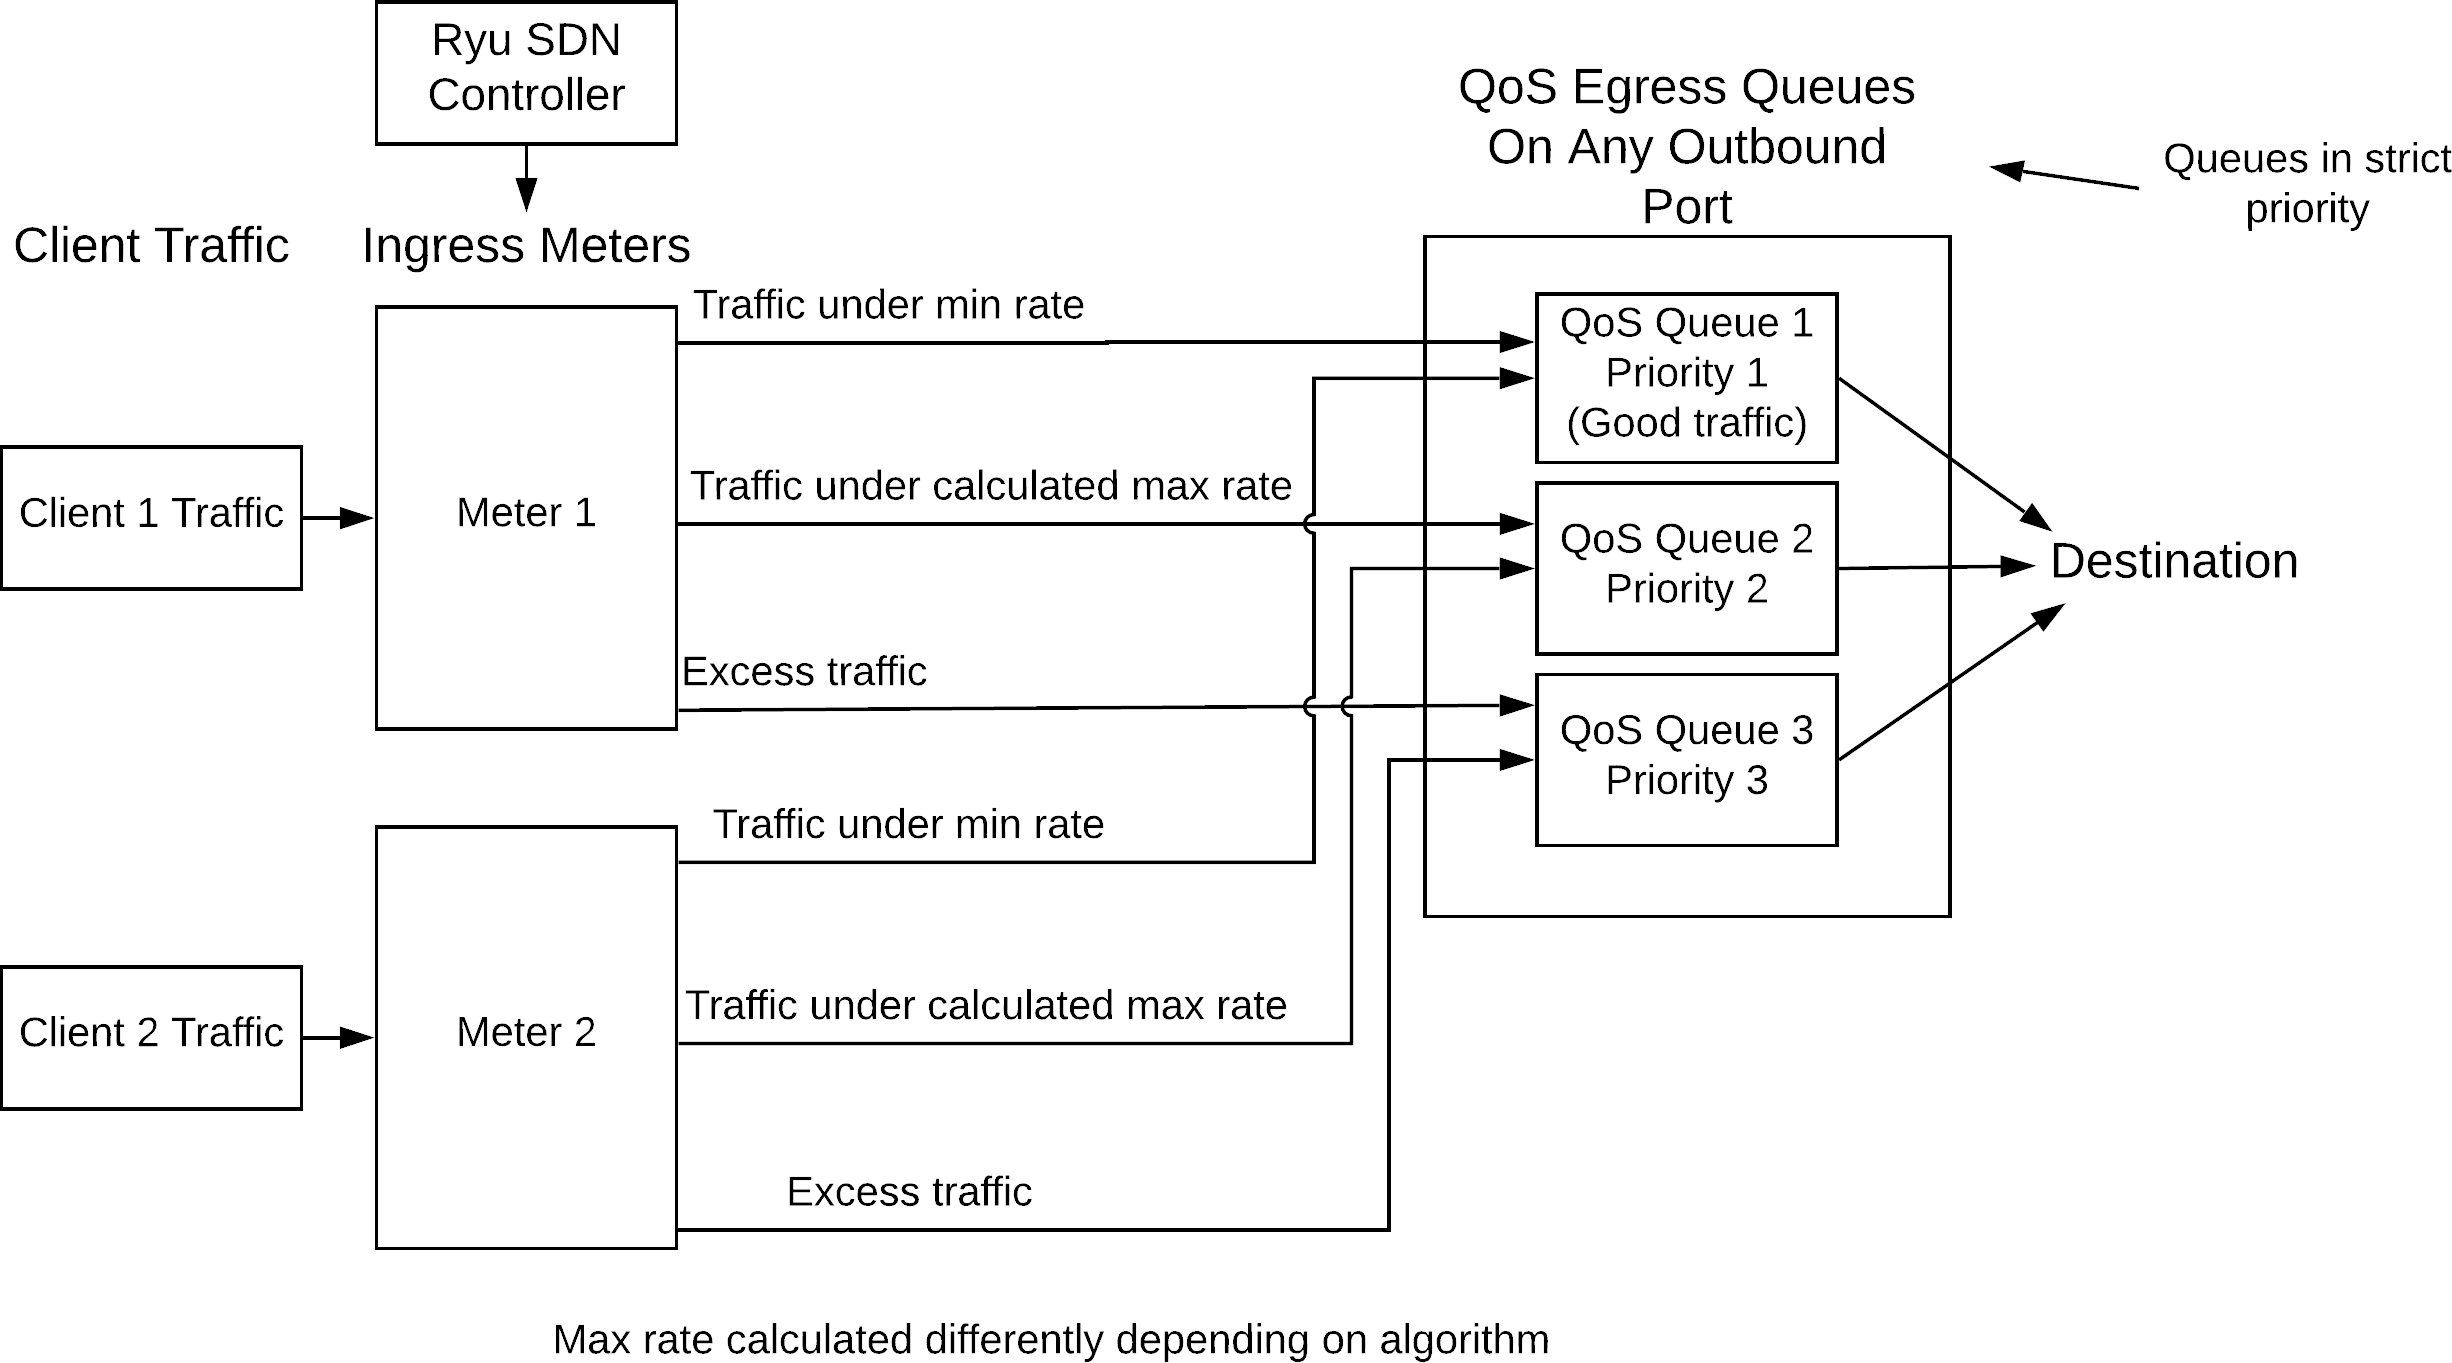
\includegraphics[width=6in]{figs/dbaFramework.png}
	\caption{ Pica8 setup with support for dynamic bandwidth allocation algorithms. } \label{dbaDiag}
\end{figure*}

EXPLAIN FIX TO THIS

The design required for bandwidth guarantees puts some restrictions on algorithm design. Only the ingress meter settings can be changed dynamically, and the egress queues must have a strict priority system, meaning the higher priority will always transmit first. This means that it is non-trivial to implement any dynamic allocation algorithm outside first-come first-serve, even an algorithm as simple as round robin will require some creativity to implement while maintaining the bandwidth guarantees. Accordingly, the three implemented allocation solutions are relatively simple: egalitarian fairness, proportional fairness, and hybrid proportional fairness.

In egalitarian fairness (Table 1), an equal share of the excess bandwidth is given to all members upon demand. This aims to treat all members as equals regardless of the minimum service they use. This solution is implemented by dividing the excess bandwidth equally between all currently active clients up to a maximum of their demand. This solution is inspired by the round robin scheduling algorithm.

\begin{table}[htpb]
	\label{egalitarian_table}
	\vspace{-3mm}
	\begin{center}
		\begin{small}
			\begin{tabular}{cccc}
				%\hline
				Client & Minimum & Demand & Allocation \\
				\hline
				Client 1 & 100 & 300 & 200 \\
				Client 2 & 200 & 400 & 300 \\
				Client 3 & 300 & 500 & 400 \\
			\end{tabular}
		\end{small}
	\end{center}
	\caption{Example of egalitarian fairness (Total bandwidth: 900 Mbps)}
	\vspace{-3mm}
\end{table}

In proportional fairness (Table 2), the share of the excess bandwidth given to each member upon demand is in proportion to its allocated minimum bandwidth guarantee. This aims to give members attributed a higher minimum service a better share of the excess bandwidth. This solution is implemented by dividing the excess bandwidth between all currently active clients up to a maximum of their demand, weighting the allocation by their minimum bandwidth. This solution is inspired by weighted round robin scheduling algorithm.

\begin{table}[htpb]
	\label{proportional_table}
	\vspace{-3mm}
	\begin{center}
		\begin{small}
			\begin{tabular}{cccc}
				%\hline
				Client & Minimum & Demand & Allocation \\
				\hline
				Client 1 & 100 & 300 & 150 \\
				Client 2 & 200 & 400 & 300 \\
				Client 3 & 300 & 500 & 450 \\
			\end{tabular}
		\end{small}
	\end{center}
	\caption{Example of proportional fairness (Total bandwidth: 900 Mbps)}
	\vspace{-3mm}
\end{table}

In hybrid proportional fairness (Table 3), each member has priority to use the excess bandwidth up to a fraction of its allocated minimum bandwidth, and the remainder is equally shared. This aims to give preference to higher usage members as in proportional fairness, but with a limitation that prevents them from dominating the channel. This solution is implemented by dividing the excess bandwidth between all currently active clients up to a maximum of their demand, starting by allocating up to 1/$X$th of their minimum bandwidth for each client, and then equally after that.

\begin{table}[h]
	\label{hybrid_table}
	\vspace{-3mm}
	\begin{center}
		\begin{small}
			\begin{tabular}{cccc}
				%\hline
				Client & Minimum & Demand & Allocation \\
				\hline
				Client 1 & 100 & 300 & 190 \\
				Client 2 & 200 & 400 & 300 \\
				Client 3 & 300 & 500 & 410 \\
			\end{tabular}
		\end{small}
	\end{center}
	\caption{Example of hybrid proportional fairness (Total bandwidth: 900 Mbps, 1/10th of minimum prioritized )}
	\vspace{-3mm}
\end{table}

In all cases all excess bandwidth is used and fairly distributed according to the algorithm's definition of fairness.

%------------------------------------------------------------------
% Results
%------------------------------------------------------------------
\section{Results}
\label{results}

Any results are currently awaiting the completed implementation and testing of the described systems. The success of the results will be evaluated by analyzing link capacity utilization and fairness of distribution.

The current expectation is that the solution will be very effective for UDP traffic and consistent traffic, but may experience performance problems with TCP traffic and bursty traffic. TCP is expected to have worse performance because the system lacks the ability to determine which packets are part of a TCP communication, and may put TCP packets in a low priority queue, leading to retransmissions. Bursty traffic is expected to have worse performance because the system is reactive, and may not be able to adjust quickly enough to be optimal for short bursts of traffic.

\subsection{Test Setups}
\label{result_setups}

testbed diagrams/explanation for why theres a loop

\subsection{Tests}
\label{result_tests}

describe the conflict and non conflict tests, that they are run on every setup
describe the over time test for dba

\subsection{No Guarantee}
\label{no_guar}

Intro of tests.

non compete

\begin{table}[h]
	\label{ng_nc}
	\vspace{-3mm}
	\begin{center}
		\begin{small}
			\begin{tabular}{cccc}
				%\hline
				Protocol & Host & Demand & Actual \\
				\hline
				UDP & Host 1 & 200 & 210\\
				    & Host 2 & 300 & 315\\
				\hline
				TCP & Host 1 & 200 & 210\\
				    & Host 2 & 300 & 315\\
			\end{tabular}
		\end{small}
	\end{center}
	\caption{Bandwidth usage for non-competing hosts in no guarantee setup.\\
	Host 1 minimum rate guarantee: 100 Mbps\\
	Host 2 minimum rate guarantee: 200 Mbps\\	
	Total available bandwidth: 600 Mbps}
	\vspace{-3mm}
\end{table}

short analysis

compete

\begin{table}[h]
	\label{ng_c}
	\vspace{-3mm}
	\begin{center}
		\begin{small}
			\begin{tabular}{cccc}
				%\hline
				Protocol & Host & Demand & Actual \\
				\hline
				UDP & Host 1 & 400 & 301\\
				    & Host 2 & 400 & 301\\
				\hline
				TCP & Host 1 & 400 & 315\\
				    & Host 2 & 400 & 277\\
			\end{tabular}
		\end{small}
	\end{center}
	\caption{Bandwidth usage for competing hosts in no guarantee setup.\\
	Host 1 minimum rate guarantee: 100 Mbps\\
	Host 2 minimum rate guarantee: 200 Mbps\\	
	Total available bandwidth: 600 Mbps}
	\vspace{-3mm}
\end{table}

short analysis

\subsection{Minimum Rate Guarantee}
\label{min_guar}

Intro of tests.

non compete

\begin{table}[h]
	\label{mg_nc}
	\vspace{-3mm}
	\begin{center}
		\begin{small}
		\setlength\tabcolsep{1.5pt}
			\begin{tabular}{cccccc}
				%\hline
				Protocol & Host & Demand & Actual & High Prio & Remarked \\
				\hline
				UDP & Host 1 & 200 & 210 & 96 & 111\\
				    & Host 2 & 300 & 315 & 192 & 119\\
				\hline
				TCP & Host 1 & 200 & 210 & 96 & 115\\
				    & Host 2 & 300 & 315 & 192 & 125\\
			\end{tabular}
		\end{small}
	\end{center}
	\caption{Bandwidth usage for non-competing hosts in minimum guarantee setup.\\
	Host 1 minimum rate guarantee: 100 Mbps\\
	Host 2 minimum rate guarantee: 200 Mbps\\	
	Total available bandwidth: 600 Mbps}
	\vspace{-3mm}
\end{table}

short analysis

compete

\begin{table}[h]
	\label{mg_c}
	\vspace{-3mm}
	\begin{center}
		\begin{small}
		\setlength\tabcolsep{1.5pt}
			\begin{tabular}{cccccc}
				%\hline
				Protocol & Host & Demand & Actual & High Prio & Remarked \\
				\hline
				UDP & Host 1 & 400 & 322 & 96 & 319\\
				    & Host 2 & 400 & 322 & 192 & 223\\
				\hline
				TCP & Host 1 & 400 & 233 & 96 & 103\\
				    & Host 2 & 400 & 359 & 191 & 145\\
			\end{tabular}
		\end{small}
	\end{center}
	\caption{Bandwidth usage for competing hosts in minimum guarantee setup.\\
	Host 1 minimum rate guarantee: 100 Mbps\\
	Host 2 minimum rate guarantee: 200 Mbps\\	
	Total available bandwidth: 600 Mbps}
	\vspace{-3mm}
\end{table}

short analysis

\subsection{Egalitarian Fairness}
\label{dba_egal}

Intro of tests.

non compete

\begin{table}[h]
	\label{egal_nc}
	\vspace{-3mm}
	\begin{center}
		\begin{small}
		\setlength\tabcolsep{1.5pt}
			\begin{tabular}{cccccccc}
				%\hline
				Protocol & Host & Demand & Expected & Actual & High & Mid & Low\\
				\hline
				UDP & Host 1 & 200 & 200 & 199 & 98 & 109 & 4\\
				    & Host 2 & 300 & 300 & 307 & 199 & 117 & 3\\
				\hline
				TCP & Host 1 & 200 & 200 & 75 & 63 & 5 & 13\\
				    & Host 2 & 300 & 300 & 315 & 199 & 127 & 1\\
			\end{tabular}
		\end{small}
	\end{center}
	\caption{Bandwidth usage for non-competing hosts in egalitarian fairness setup.\\
	Host 1 minimum rate guarantee: 100 Mbps\\
	Host 2 minimum rate guarantee: 200 Mbps\\	
	Total available bandwidth: 600 Mbps}
	\vspace{-3mm}
\end{table}

short analysis

compete

\begin{table}[h]
	\label{egal_c}
	\vspace{-3mm}
	\begin{center}
		\begin{small}
		\setlength\tabcolsep{1.5pt}
			\begin{tabular}{cccccccc}
				%\hline
				Protocol & Host & Demand & Expected & Actual & High & Mid & Low\\
				\hline
				UDP & Host 1 & 400 & 250 & 242 & 98 & 178 & 175\\
				    & Host 2 & 400 & 350 & 370 & 197 & 175 & 38\\
				\hline
				TCP & Host 1 & 400 & 250 & 85 & 73 & 6 & 14\\
				    & Host 2 & 400 & 350 & 419 & 197 & 234 & 3\\
			\end{tabular}
		\end{small}
	\end{center}
	\caption{Bandwidth usage for competing hosts in egalitarian fairness setup.\\
	Host 1 minimum rate guarantee: 100 Mbps\\
	Host 2 minimum rate guarantee: 200 Mbps\\	
	Total available bandwidth: 600 Mbps}
	\vspace{-3mm}
\end{table}

short analysis

Over time graphs

short analysis

\subsection{Proportional Fairness}
\label{dba_prop}
Intro of tests.

non compete

\begin{table}[h]
	\label{prop_nc}
	\vspace{-3mm}
	\begin{center}
		\begin{small}
		\setlength\tabcolsep{1.5pt}
			\begin{tabular}{cccccccc}
				%\hline
				Protocol & Host & Demand & Expected & Actual & High & Mid & Low\\
				\hline
				UDP & Host 1 & 200 & 200 & 199 & 98 & 109 & 4\\
				    & Host 2 & 300 & 300 & 308 & 198 & 118 & 2\\
				\hline
				TCP & Host 1 & 200 & 200 & 86 & 78 & 5 & 15\\
				    & Host 2 & 300 & 300 & 314 & 197 & 96 & 19\\
			\end{tabular}
		\end{small}
	\end{center}
	\caption{Bandwidth usage for non-competing hosts in proportional fairness setup.\\
	Host 1 minimum rate guarantee: 100 Mbps\\
	Host 2 minimum rate guarantee: 200 Mbps\\	
	Total available bandwidth: 600 Mbps}
	\vspace{-3mm}
\end{table}

short analysis

compete

\begin{table}[h]
	\label{prop_c}
	\vspace{-3mm}
	\begin{center}
		\begin{small}
		\setlength\tabcolsep{1.5pt}
			\begin{tabular}{cccccccc}
				%\hline
				Protocol & Host & Demand & Expected & Actual & High & Mid & Low\\
				\hline
				UDP & Host 1 & 400 & 200 & 198 & 98 & 102 & 223\\
				    & Host 2 & 400 & 400 & 397 & 197 & 207 & 13\\
				\hline
				TCP & Host 1 & 400 & 200 & 91 & 73 & 6 & 14\\
				    & Host 2 & 400 & 400 & 419 & 197 & 235 & 2\\
			\end{tabular}
		\end{small}
	\end{center}
	\caption{Bandwidth usage for competing hosts in proportional fairness setup.\\
	Host 1 minimum rate guarantee: 100 Mbps\\
	Host 2 minimum rate guarantee: 200 Mbps\\	
	Total available bandwidth: 600 Mbps}
	\vspace{-3mm}
\end{table}

short analysis

Over time graphs

short analysis

\subsection{Hybrid Proportional Fairness}
\label{dba_hybr}
Intro of tests.

non compete

\begin{table}[h]
	\label{hybr_nc}
	\vspace{-3mm}
	\begin{center}
		\begin{small}
		\setlength\tabcolsep{1.5pt}
			\begin{tabular}{cccccccc}
				%\hline
				Protocol & Host & Demand & Expected & Actual & High & Mid & Low\\
				\hline
				UDP & Host 1 & 200 & 200 & 201 & 98 & 110 & 3\\
				    & Host 2 & 300 & 300 & 309 & 199 & 120 & 1\\
				\hline
				TCP & Host 1 & 200 & 200 & 103 & 75 & 15 & 17\\
				    & Host 2 & 300 & 300 & 315 & 197 & 128 & 0\\
			\end{tabular}
		\end{small}
	\end{center}
	\caption{Bandwidth usage for non-competing hosts in hybrid proportional fairness setup.\\
	1/10th of minimum prioritized\\	
	Host 1 minimum rate guarantee: 100 Mbps\\
	Host 2 minimum rate guarantee: 200 Mbps\\	
	Total available bandwidth: 600 Mbps}
	\vspace{-3mm}
\end{table}

short analysis

compete

\begin{table}[h]
	\label{hybr_c}
	\vspace{-3mm}
	\begin{center}
		\begin{small}
		\setlength\tabcolsep{1.5pt}
			\begin{tabular}{cccccccc}
				%\hline
				Protocol & Host & Demand & Expected & Actual & High & Mid & Low\\
				\hline
				UDP & Host 1 & 400 & 245 & 238 & 98 & 149 & 180\\
				    & Host 2 & 400 & 355 & 369 & 197 & 170 & 37\\
				\hline
				TCP & Host 1 & 400 & 245 & 80 & 67 & 5 & 13\\
				    & Host 2 & 400 & 355 & 419 & 198 & 236 & 4\\
			\end{tabular}
		\end{small}
	\end{center}
	\caption{Bandwidth usage for competing hosts in hybrid proportional fairness setup.\\
	1/10th of minimum prioritized\\
	Host 1 minimum rate guarantee: 100 Mbps\\
	Host 2 minimum rate guarantee: 200 Mbps\\	
	Total available bandwidth: 600 Mbps}
	\vspace{-3mm}
\end{table}

short analysis

Over time graphs

short analysis

\subsection{Overall Result Analysis}
\label{result_analysis}

UDP good
TCP bad


%------------------------------------------------------------------
% Discussion
%------------------------------------------------------------------
\section{Discussion}
\label{discussion}

Any substantial discussion is currently awaiting the completed implementation and testing of the described systems.

Overall, is the approach we took promising?
What different approach or variant of this approach is better?
What follow-up work should be done next?
What did we learn by doing this project?

%------------------------------------------------------------------
% Conclusion
%------------------------------------------------------------------
\section{Conclusion}
\label{conclusion}

Any substantial conclusion is currently awaiting the completed implementation and testing of the described systems.

%------------------------------------------------------------------
% Bibliography
%------------------------------------------------------------------
\bibliography{refs}

\end{document}
